\documentclass[11pt]{article}
\usepackage[paperwidth=7.5in,paperheight=10.5in,inner=.79in,outer=.72in,top=.79in,bottom=.78in]{geometry}
\usepackage[T1]{fontenc}
\usepackage{amsmath,amsthm}
\usepackage{newpxtext,newpxmath,microtype}
\usepackage{booktabs,array,graphicx,xcolor,fancyhdr,titlesec,hyperref,enumitem}
\definecolor{PhysicsNavy}{HTML}{142D40}
\definecolor{PhysicsTeal}{HTML}{176974}
\definecolor{PhysicsCopper}{HTML}{A67B50}
\hypersetup{colorlinks=true,linkcolor=PhysicsTeal,citecolor=PhysicsTeal,urlcolor=PhysicsTeal,pdftitle={Energy-Conserving Production},pdfauthor={Komorebi P.}}
\setlength{\parindent}{1.1em}\setlength{\parskip}{.22em}
\setlength{\headheight}{15pt}
\pagestyle{fancy}\fancyhf{}
\fancyhead[L]{\footnotesize\sffamily\color{PhysicsTeal}KOMOREBI PHYSICS}
\fancyhead[R]{\footnotesize\sffamily ENERGY-CONSERVING PRODUCTION}
\fancyfoot[R]{\thepage}
\renewcommand{\headrulewidth}{.3pt}
\titleformat{\section}{\Large\bfseries\color{PhysicsNavy}}{\thesection}{.6em}{}
\titleformat{\subsection}{\large\bfseries\color{PhysicsTeal}}{\thesubsection}{.6em}{}
\titlespacing*{\section}{0pt}{1.6em}{.6em}
\titlespacing*{\subsection}{0pt}{1.1em}{.4em}
\newtheorem{theorem}{Theorem}[section]
\newtheorem{proposition}[theorem]{Proposition}
\newtheorem{corollary}[theorem]{Corollary}
\theoremstyle{definition}\newtheorem{definition}[theorem]{Definition}
\newcommand{\dd}{\mathrm d}\newcommand{\eps}{\varepsilon}
\newcommand{\rhoV}{\rho_{\mathrm V}}
\newcommand{\e}{\mathrm e}
\graphicspath{{figures/}}
\begin{document}
\thispagestyle{empty}
{\noindent\sffamily\small\color{PhysicsTeal}OPERATION KOMOREBI\hfill MATHEMATICAL PHYSICS\par}
\vspace{.55in}
{\noindent\fontsize{31}{36}\selectfont\bfseries\color{PhysicsNavy}Energy-Conserving\\Production\par}
\vspace{.20in}
{\noindent\Large A finite-depth backreaction study\par}
\vspace{.19in}
{\noindent\color{PhysicsCopper}\rule{1.25in}{1pt}\par}
\vspace{.16in}
\noindent The crossing-energy obstruction, an abundance-preserving parameter family, and a quantum-mode calculation with explicit energy exchange.\par
\vspace{.28in}
\noindent\textbf{Komorebi P.}\hfill October 2026\par
\vspace{.35in}
\noindent\textbf{Result and boundary.} The original prescribed-background benchmark exceeds its crossing reservoir by $2.6272875374\times10^{20}$. This study constructs a finite dynamical system in which that kind of overdraw is excluded by an exact conservation law. A numerical implementation agrees with an independent oscillator representation and conserves its total energy to the stated tolerance.

The calculation does \emph{not} recover the cosmological benchmark. It uses a finite cutoff and a specified instantaneous vacuum. Its dependence on tower depth and momentum cutoff remains substantial. A separate analytic parameter family removes the Gaussian energy overdraw without multiplying occupations by an arbitrary factor, but it creates a larger residual background reservoir and does not remove the tower's radiative sensitivity.

These are distinct outcomes: a closed conservation result for the finite model, a conditional parameter construction, and a failed test of cutoff independence. None is labeled a renormalized cosmological solution or a new Lean certificate.
\vfill
{\noindent\footnotesize Original text and figures: CC BY 4.0. Original accompanying software: MIT. The existing physics monograph is unchanged by this research study.\par}
\clearpage

\section{The obstruction being addressed}
The source model is a real background scalar coupled to a finite tower of real scalar fields. In the massless-base benchmark,
\begin{align}
 U(\phi)&=\frac{\lambda}{4}(\phi^2-v^2)^2,
 &\mu^2&=\lambda v^2,\\
 m_h&=\Lambda 2^h,
 &d_h&=2^{h-1},\\
 M_h^2(\phi)&=m_h^2\left(1+\gamma\frac{\phi^2}{v^2}\right),
 &\gamma&=16.
\end{align}
The general covariant construction and its limitations are given in the source monograph \cite{komorebi}. This study fixes the dyadic order-one tower used in the stored benchmark. The quartic $\lambda$ is not a spectral eigenvalue.

For a prescribed locally linear crossing, put
\begin{equation}
 A=\frac{\sqrt\gamma\,|\dot\phi_\star|}{v},\qquad
 x=\frac\Lambda A=10^{-4},\qquad y_h=\frac{m_h}{A}=x2^h.
\end{equation}
The assumed single-crossing occupation is
\begin{equation}
 f_h(k)=\exp\!\left[-\pi\left(\frac{m_h}{A}+\frac{k^2}{Am_h}\right)\right].
 \label{eq:gaussian}
\end{equation}
Such a prescribed crossing does not account for depletion of its source. The distinction between prescribed production, particle-mass growth, and self-consistent reaction is also central in established preheating calculations \cite{kls,instant}.

Write the energy evaluated with the minimum masses as
\begin{equation}
 \widetilde\rho=A^4 S_E(x),\qquad S_E(10^{-4})=2.18498795564,
 \label{eq:SE}
\end{equation}
where the exact discrete degeneracies are retained. The kinetic reservoir is
\begin{equation}
 K=\frac{v^2 A^2}{2\gamma},\qquad
 \rhoV=\frac{\mu^4}{4\lambda},\qquad
 \frac K{\rhoV}=\frac{2}{\gamma}\left(\frac A\mu\right)^2.
 \label{eq:kinetic}
\end{equation}
The stored reference has $\lambda_0=1$ and
\begin{align}
 a_0:=\frac{A_0}{\mu_0}&=1.93844860142\times10^9,\\
 \frac{K_0}{\rhoV}&=4.69697872544\times10^{17},\\
 R_0:=\frac{\widetilde\rho_0}{K_0}
 &=2.6272875374\times10^{20}.
\end{align}
The original occupation projection used
\begin{equation}
 \eta_0=R_0^{-1}=3.80620691783\times10^{-21}.
 \label{eq:eta}
\end{equation}
It made the reported density equal to $K_0$, but did not supply equations that remove this energy from the evolving scalar.

The inherited verification program was rerun: all 19 checks passed within their declared scope. An independent adaptive momentum integral was also compared with its generalized Laguerre integral. The supplied JSON preserves the full numerical residuals. Passing this arithmetic audit confirms the obstruction; it does not validate the physical production history.

\section{Removing overdraw inside the Gaussian family}
Simply reducing $\lambda$ at fixed $A/\mu$ reduces both the overdraw and the output density relative to the old target. To preserve the target density while imposing a smaller nominal conversion fraction, the crossing scale in units of $\mu$ must change too.

\begin{theorem}[Conditional abundance-preserving family]
Fix $\rhoV$, $\gamma$, the tower order, and $x=\Lambda/A$. Let the target density be the original projected value $\rho_T=\eta_0 A_0^4 S_E=K_0$. For any $0<\eps\le1$, choose
\begin{equation}
 \boxed{\lambda=\eta_0\eps^2,\qquad
 \frac A\mu=\frac{a_0}{\sqrt\eps},\qquad
 \frac\Lambda\mu=x\frac{a_0}{\sqrt\eps}.}
 \label{eq:family}
\end{equation}
Then the unprojected Gaussian family satisfies
\begin{equation}
 \widetilde\rho=\rho_T,\qquad
 K=\frac{K_0}{\eps},\qquad
 \frac{\widetilde\rho}{K}=\eps.
 \label{eq:familyresult}
\end{equation}
No common occupation multiplier is used in this construction.
\end{theorem}
\begin{proof}
At fixed $\rhoV$, $\mu^4=4\lambda\rhoV$, so
\[
 \widetilde\rho=4\rhoV\lambda(A/\mu)^4S_E.
\]
Substitute \eqref{eq:family}. The factors $\eps^2$ and $\eps^{-2}$ cancel, leaving $\eta_0 A_0^4S_E$. Equation \eqref{eq:kinetic} gives $K=K_0/\eps$. Division proves the final identity.
\end{proof}

Here $\eps$ is a \emph{design parameter for the stipulated Gaussian family}. It is not the measured production efficiency of the coupled solver below. That solver includes coherent vacuum response and changes the trajectory.

\subsection{What is and is not preserved}
The density and the normalized distributions in $m/A$ and $k/A$ are preserved. The physical mass scale is not the old one:
\begin{equation}
 \frac\mu{\mu_0}=\eta_0^{1/4}\sqrt\eps,\qquad
 \frac A{A_0}=\frac\Lambda{\Lambda_0}=\eta_0^{1/4}
 =7.85458237208\times10^{-6}.
 \label{eq:physicalscale}
\end{equation}
Thus the physical tower masses are independent of $\eps$ along this family, but differ from the original projected benchmark. Number density increases by the inverse of the common mass factor, while the mass density is held fixed. Occupations themselves are not preserved: they are no longer multiplied by $\eta_0$.

The canonical coupling of level $h$ is
\begin{equation}
 g_h=\gamma\lambda\left(\frac{m_h}{\mu}\right)^2.
\end{equation}
At the stored peak level $h=13$, this becomes
\begin{equation}
 g_{\rm peak}=0.1535680410\,\eps.
\end{equation}
The following numbers are algebraic consequences of the parameter choice, not fitted dynamical outputs.

\begin{center}\small
\begin{tabular}{@{}rrrr@{}}\toprule
$\eps$ & $\lambda$ & $g_{\rm peak}$ & $K/K_0$\\\midrule
1 & $3.8062\times10^{-21}$ & $0.15357$ & 1\\
0.1 & $3.8062\times10^{-23}$ & $0.015357$ & 10\\
0.03 & $3.4256\times10^{-24}$ & $0.0046070$ & $33.333$\\
0.01 & $3.8062\times10^{-25}$ & $0.0015357$ & 100\\
0.003 & $3.4256\times10^{-26}$ & $0.00046070$ & $333.333$\\
\bottomrule\end{tabular}
\end{center}

\section{The reservoir cannot be ignored}
\begin{proposition}[Residual-energy obligation]
Suppose an event begins and ends at the same scalar potential value, expansion and external losses are negligible during that event, and the receiving sector gains $\eps K_i$. Energy conservation requires
\begin{equation}
 K_f=(1-\eps)K_i.
\end{equation}
In particular, weak transfer in that event cannot also bring the background to rest at the same potential value without another energy-transfer mechanism.
\end{proposition}
\begin{proof}
Subtract the initial and final conserved total energies. The potential contributions cancel. The gain in receiving-sector energy is the loss in kinetic energy.
\end{proof}

At $\eps=0.01$, the Gaussian bookkeeping leaves 99 percent of the incident kinetic energy outside the target produced density. This is not automatically an inconsistency. Further mass growth, subsequent passages, expansion, or transfer to other fields can act. But their effect must be computed, and they need not preserve the stipulated spectrum. Mass growth after a crossing can itself transfer substantial energy \cite{instant}.

There is also a quantitative background cost. Using the \emph{stored benchmark inputs}, not a new observational fit,
\begin{equation}
 a_\star=10^{-6},\quad \Omega_{r0}=9\times10^{-5},\quad
 \Omega_{\mathrm V}=0.68991,
\end{equation}
we obtain
\begin{equation}
 \boxed{\frac{K}{\rho_r(a_\star)}=\frac{0.003600547325}{\eps}.}
 \label{eq:radiation}
\end{equation}
The ratio is $0.0360$ at $\eps=0.1$, $0.360$ at $0.01$, and $3.60$ at $0.001$. Taking $\eps$ arbitrarily small is therefore not a cost-free way to preserve the old cosmological history. These ratios are not observational exclusion bounds. They identify a background component that the next cosmological calculation must include.

\section{A finite quantum system with an exact energy budget}
\subsection{Regulator and state}
Set
\begin{equation}
 q=\frac{\sqrt\gamma\phi}{v},\quad \tau=At,\quad
 \kappa=\frac{k}{A},\quad
 \omega_{h\kappa}(q)=\sqrt{\kappa^2+y_h^2(1+q^2)}.
\end{equation}
After finite momentum quadrature, label a mode by $j$ and give it a positive weight $w_j$, including its tower multiplicity. Let
\begin{equation}
 C=\frac{v^2}{\gamma A^2}
 =\frac{1}{\gamma\lambda(A/\mu)^2}
 =\frac{2S_E}{\eps}>0.
\end{equation}
The prime in the rest of this section denotes $\dd/\dd\tau$.

For each mode use the instantaneous occupation $n_j$ and two real coherence variables $u_j,v_j$. They obey
\begin{align}
 n_j'&=\frac12 W_j u_j,\\
 u_j'&=W_j(1+2n_j)-2\omega_j v_j,\\
 v_j'&=2\omega_j u_j,\qquad
 W_j=\frac{\omega_{j,q}q'}{\omega_j}.
 \label{eq:qke}
\end{align}
These equations are the oscillator Bogoliubov system in real variables. Quantum-kinetic and scattering descriptions of time-dependent pair production are closely related \cite{qke}. Their use here is defined directly by the finite oscillator model, not by importing an electromagnetic pair-production claim into the scalar model.

The reaction force required by the same finite Hamiltonian is
\begin{equation}
 \boxed{Cq''+\mathcal V'(q)
 +\sum_j w_j\omega_{j,q}\left(n_j+\frac{u_j}{2}\right)=0.}
 \label{eq:reaction}
\end{equation}
The coherence term is essential. An occupation-only force does not conserve the energy of \eqref{eq:qke}.

\subsection{Precise subtraction convention}
For complex mode functions $a_j$ satisfying $a_j''+\omega_j^2a_j=0$ and the normalization $a_j\overline{a_j'}-\overline{a_j}a_j'=i$, fix the variables by
\begin{equation}
 n_j=\frac{|a_j'|^2+\omega_j^2|a_j|^2}{2\omega_j}-\frac12,
 \quad u_j=\omega_j|a_j|^2-\frac{|a_j'|^2}{\omega_j},
 \quad v_j=-2\operatorname{Re}(\overline{a_j}a_j').
\end{equation}
Use the finite energy
\begin{equation}
 \mathcal E=\frac C2(q')^2+\mathcal V(q)
 +\sum_jw_j\left[\frac{|a_j'|^2+\omega_j^2|a_j|^2}{2}
 -\frac{\omega_j}{2}\right].
 \label{eq:hamiltonian}
\end{equation}
The subtracted quantity depends on $q$, so its derivative must also be included in the force. This gives \eqref{eq:reaction}. The bracket in \eqref{eq:hamiltonian} equals $\omega_jn_j$.

This is a \emph{finite instantaneous zero-point subtraction}, specified as part of the regulated Hamiltonian. It is not a completed covariant adiabatic-renormalization prescription, nor a proof that a chosen continuum renormalization condition produces the same effective potential. Renormalized semiclassical energy and force terms must be obtained consistently; conservation of the complete stress tensor is the relevant condition \cite{mpr,psar}.

\begin{theorem}[Finite energy conservation and positivity]
Assume $C>0$, $w_j>0$, $y_j>0$, and $\mathcal V\ge0$ is smooth. Start the modes in the instantaneous vacuum $n_j=u_j=v_j=0$. Equations \eqref{eq:qke}--\eqref{eq:reaction} preserve
\begin{equation}
 (1+2n_j)^2-u_j^2-v_j^2=1,
 \label{eq:hyperboloid}
\end{equation}
and conserve
\begin{equation}
 \boxed{\mathcal E=\frac C2(q')^2+\mathcal V(q)
 +\sum_jw_j\omega_j n_j.}
 \label{eq:conserved}
\end{equation}
Every occupation remains nonnegative. Consequently
\begin{equation}
 0\le\sum_jw_j\omega_j n_j\le\mathcal E(0).
 \label{eq:bound}
\end{equation}
\end{theorem}
\begin{proof}
Differentiate the left side of \eqref{eq:hyperboloid} and substitute \eqref{eq:qke}; all terms cancel. The initial value is one. The continuous trajectory remains on the sheet $1+2n_j>0$, which implies $1+2n_j\ge1$ and hence $n_j\ge0$.

For the mode energy,
\[
 (\omega_jn_j)'=\omega_{j,q}q'\left(n_j+\frac{u_j}{2}\right).
\]
Multiplying \eqref{eq:reaction} by $q'$ cancels the sum of these derivatives against the derivative of the mechanical energy. This proves \eqref{eq:conserved}. Its nonnegative terms prove \eqref{eq:bound}.
\end{proof}

\begin{corollary}[Global existence at fixed finite regulator]
Under the theorem's assumptions, the finite initial-value problem has a unique solution for all finite times.
\end{corollary}
\begin{proof}
The vector field is smooth because each $\omega_j$ is bounded below by $y_j>0$. Conservation bounds $q'$, so $q$ stays bounded on every finite time interval. Positivity bounds $n_j\le\mathcal E(0)/(w_jy_j)$, and \eqref{eq:hyperboloid} then bounds both coherence variables. The ordinary differential equation cannot leave every compact subset in finite time. The local solution therefore extends globally.
\end{proof}

This is the exact sense in which the finite model resolves energy overdraw. It does not establish that the chosen regulator, subtraction, initial state, or spectrum is the physical completion of the cosmological proposal.

\section{Numerical results and tests that failed}
The principal run takes $\eps=0.01$, depth 16, 48 Gauss--Legendre momentum nodes per level, and
\begin{equation}
 \kappa=\sqrt{y_h}\,z,\quad 0\le z\le3.5,\quad
 q(0)=-10,\quad q'(0)=1,\quad 0\le\tau\le20.
\end{equation}
Here $A$ is the nominal reference scale used to set the incoming speed. The actual speed at $q=0$ is an output of the coupled solution, not an imposed crossing condition. There are 768 quadrature modes, representing 65,535 internal scalar degrees of freedom. The modes begin in the specified instantaneous vacuum. We use $\mathcal V=0$ as a local crossing diagnostic. For the nominal parameter family and $|q|\le10$, the original quartic potential energy is below $6\times10^{-19}$ of the crossing kinetic reservoir. That local estimate is not permission to omit the potential from the subsequent trapping calculation.

The DOP853 integration uses relative tolerance $2\times10^{-10}$ and absolute tolerance $2\times10^{-13}$. The largest total-energy residual in the principal run is
\begin{equation}
 \max_\tau\left|\frac{\mathcal E(\tau)}{\mathcal E(0)}-1\right|
 =7.34\times10^{-11}.
\end{equation}
The maximum hyperboloid residual is $3.73\times10^{-13}$. The largest instantaneous mode-energy fraction is $0.648634$, and the endpoint fraction is $0.126747$. The final position is $q=6.65567$, rather than the externally forced value $q=10$.

\begin{figure}[htbp]\centering
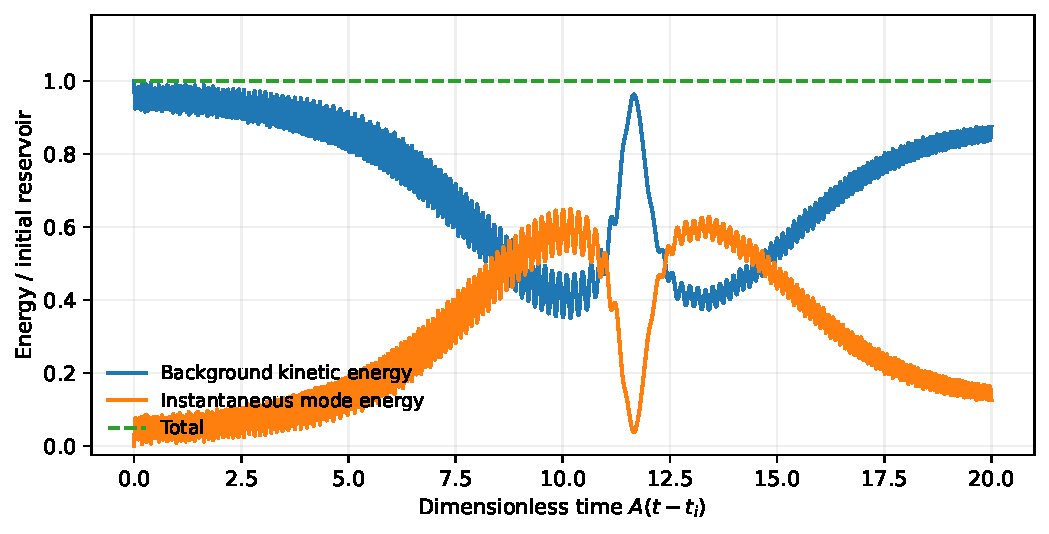
\includegraphics[width=\linewidth]{conserved_energy.pdf}
\caption{Energy is exchanged with the background rather than added to a prescribed trajectory. The mode energy includes instantaneous-basis vacuum response. It is not an asymptotic dark-particle yield.}
\end{figure}

The difference between the nominal Gaussian fraction of one percent and these larger transient fractions is not an improved abundance prediction. The finite system contains coherent vacuum response, and its initial-state and cutoff choices are not yet a renormalized continuum construction.

\subsection{Independent representation and numerical resolution}
A separately coded complex-oscillator system was compared with the real quantum-kinetic implementation at depth 14, with 12 nodes and a shorter interval. Their maximum background-position difference was $1.88\times10^{-10}$; their maximum mode-energy-fraction difference was $1.71\times10^{-9}$. This checks the change of variables and reaction-force implementation. It is not an independent physical model.

At the principal cutoff, increasing momentum quadrature from 48 to 64 nodes leaves the reported endpoint fraction $0.12674744$ unchanged at the displayed precision. This is \emph{quadrature convergence at fixed cutoff}. It must not be confused with cutoff independence.

\subsection{Negative controls}
Two incorrect closed-system variants were run. Omitting the entire reaction force gives a maximum total-energy residual of $1.47269$ relative to the initial reservoir. Keeping only the occupation force and discarding coherence gives a residual of $5.29845$. The full system has neither defect.

An externally prescribed trajectory can consistently be interpreted as receiving external work. The first negative control is wrong only when it is presented as a \emph{closed} system with the old finite reservoir. This is precisely the bookkeeping assumption tested here.

\begin{figure}[htbp]\centering
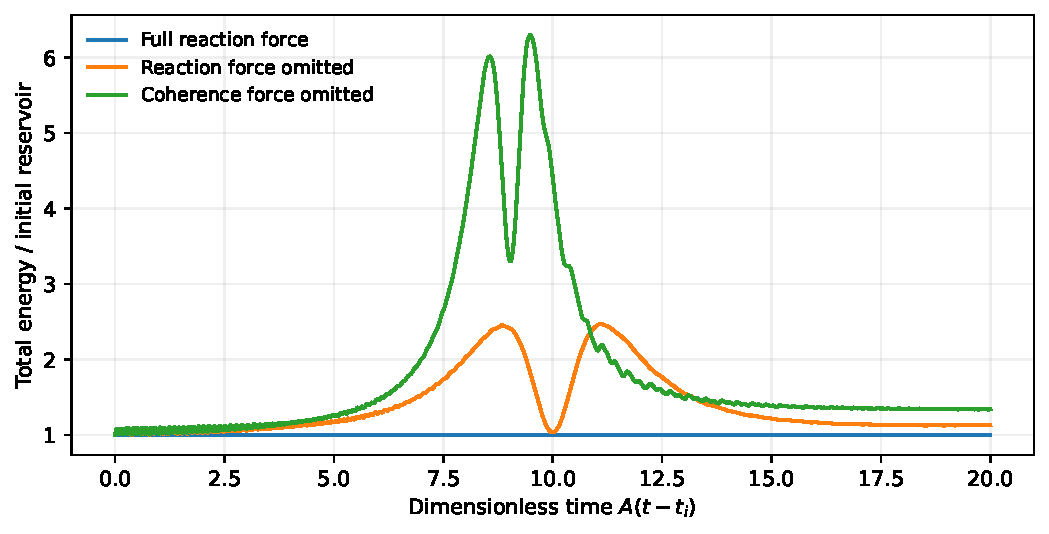
\includegraphics[width=\linewidth]{negative_controls.pdf}
\caption{Deleting either necessary reaction term destroys the stated closed-system budget. The controls test the conservation mechanism, not a universal physical model.}
\end{figure}

\subsection{The cutoff test does not pass}
Increasing depth changes the regulated Hamiltonian, not merely the quadrature accuracy. Nevertheless, an interpretation that removes the depth regulator must establish stability under that change. The present system does not do so:
\begin{center}\small
\begin{tabular}{@{}rrr@{}}\toprule
Depth & Maximum instantaneous mode fraction & Final $q$\\\midrule
14 & 0.079418 & 9.59614\\
15 & 0.245202 & 8.93592\\
16 & 0.648634 & 6.65567\\
17 & 0.940562 & 2.18787\\
18 & 0.9999998 & $-0.75818$\\\bottomrule
\end{tabular}\end{center}
All rows use the same time interval, not a common outgoing field position. The last row is not even on the positive side at the final time. These fractions are not comparable asymptotic particle yields.

At depth 16, changing $z_{\max}$ from 2.5 to 3.5 to 4.5 to 6 changes the maximum mode-energy fraction from approximately 0.476 to 0.649 to 0.762 to 0.871. Moving the initial state from $q=-10$ to $-15$ or $-20$ also changes the endpoint result. Thus the failed scientific gate is genuine. Conservation has passed; regulator and state robustness have not.

\begin{figure}[htbp]\centering
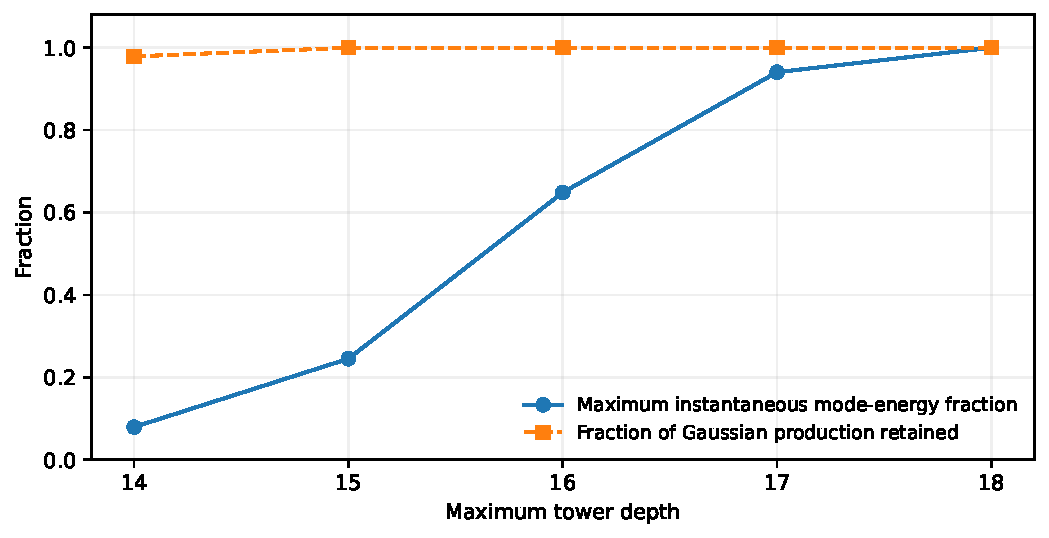
\includegraphics[width=\linewidth]{depth_sensitivity.pdf}
\caption{The Gaussian production sum is already almost saturated while the finite quantum response continues to change. Production-tail truncation is not a sufficient ultraviolet justification for a dynamical calculation.}
\end{figure}

The 17-run study includes two negative controls and resolution, cutoff, endpoint, and coupling variations. The verification summary records 11 passing algebraic or numerical gates and one failed scientific gate. The failure is not relabeled as a successful regression.

\section{Why a smaller coupling is not a complete repair}
\subsection{A radiative quantity invariant along the abundance family}
The source monograph gives the finite-depth one-loop curvature contribution with its subtraction-scale logarithms. To isolate power counting, define the nonnegative diagnostic
\begin{equation}
 \mathcal N_H:=\frac{\gamma\lambda}{16\pi^2}
 \sum_{h=1}^H d_h\left(\frac{m_h}{\mu}\right)^4.
 \label{eq:curvatureproxy}
\end{equation}
This omits logarithms and finite counterterms. It is neither a scheme-independent lower bound on the renormalized mass nor a proof that locking is impossible.

\begin{proposition}[Invariant curvature power counting]
At fixed $\rhoV$ and $\gamma$, the family \eqref{eq:family} leaves $\mathcal N_H$ unchanged for each fixed depth:
\begin{equation}
 \mathcal N_H
 =\frac{\gamma\eta_0 a_0^4}{16\pi^2}\sum_{h=1}^H d_hy_h^4
 =\frac{\gamma}{64\pi^2\rhoV}\sum_{h=1}^H d_hm_h^4.
\end{equation}
\end{proposition}
\begin{proof}
The factor $\lambda(A/\mu)^4$ equals $\eta_0a_0^4$ by \eqref{eq:family}. Equivalently, substitute $\mu^4=4\lambda\rhoV$ into \eqref{eq:curvatureproxy}. The physical masses are fixed along the family by \eqref{eq:physicalscale}.
\end{proof}

The values are about $1.04\times10^{19}$ through depth 13, $1.06\times10^{22}$ through depth 15, and $3.40\times10^{23}$ through depth 16. Depth 15 already contains $99.9992126$ percent of the stipulated Gaussian energy. Making individual couplings smaller does not, on this slice, remove the required relative curvature tuning or protection.

\begin{figure}[htbp]\centering
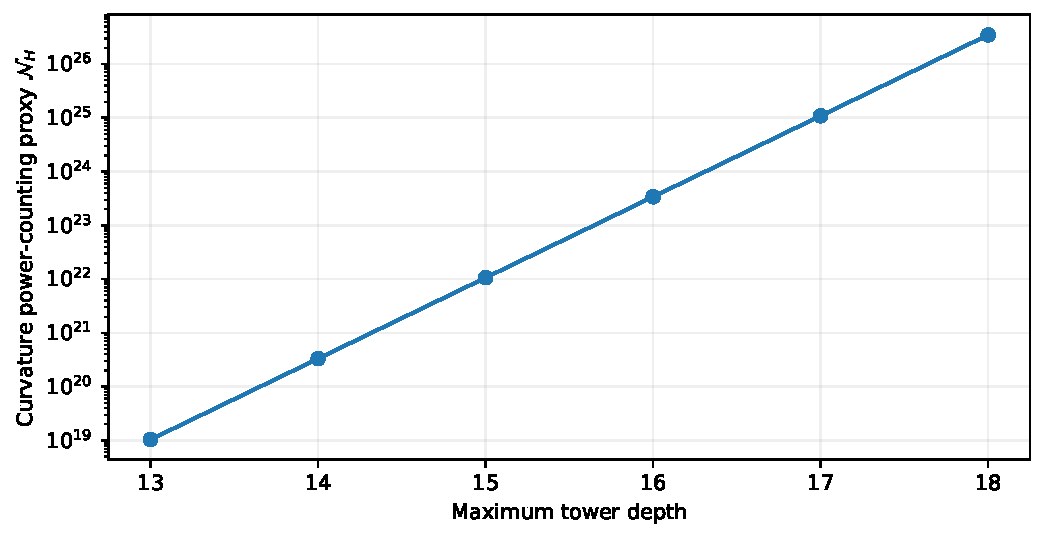
\includegraphics[width=\linewidth]{radiative_proxy.pdf}
\caption{The curvature power-counting diagnostic grows with the fourth mass moment. It is independent of the nominal Gaussian depletion parameter along the abundance-preserving family. Logarithms and counterterms are not represented by this diagnostic.}
\end{figure}

This leaves genuine choices: explicitly matched finite-cutoff counterterms, a protected matter completion, or different microscopic production parameters and observables. It does not support the claim that arbitrarily small $\lambda$ alone has made the model radiatively natural.

\subsection{Vacuum response from unproduced levels}
The observed depth sensitivity has a useful analytic warning sign. In a sufficiently adiabatic mode,
\begin{equation}
 n^{(2)}\simeq\frac{(\omega')^2}{16\omega^4},\qquad
 \omega n^{(2)}\simeq\frac{y^4q^2(q')^2}{16\omega^5}.
\end{equation}
Integrating this local second-adiabatic-order energy over the full momentum range gives
\begin{equation}
 \mathcal E^{(2)}_H
 =\frac{(q')^2}{96\pi^2}\frac{q^2}{1+q^2}
 \sum_{h=1}^H d_hy_h^2,
 \label{eq:adiabatice}
\end{equation}
because
\[
 \int_0^\infty\frac{\kappa^2\,\dd\kappa}{(\kappa^2+M^2)^{5/2}}
 =\frac{1}{3M^2}.
\]
It therefore corresponds to the local kinetic correction
\begin{equation}
 \delta C_H(q)=\frac{1}{48\pi^2}\frac{q^2}{1+q^2}
 \sum_{h=1}^H d_hy_h^2.
\end{equation}
At large $|q|$, $\delta C_H/C$ for $\eps=0.01$ is approximately 0.121 at depth 14, 0.971 at 15, 7.77 at 16, and 62.2 at 17.

Equation \eqref{eq:adiabatice} is an adiabatic diagnostic, not an exact explanation of every transient or a subtraction inserted into the numerical solver. Low modes near a nonadiabatic crossing need the full dynamics. Its significance is narrower: a high level can be exponentially irrelevant to \eqref{eq:gaussian} yet still matter to vacuum response. A physical depth endpoint or a matched ultraviolet prescription cannot be replaced by the cutoff used merely to sum real production.

\section{The next decisive calculation}
The finite result closes the mathematical bookkeeping defect but leaves the physical selection of the theory open. A defensible continuation starts with a declared physical depth or ultraviolet completion, a covariantly consistent subtraction prescription, fixed renormalization conditions, and an appropriate incoming state. The same prescription must determine the background force, energy, pressure, and gravitational equations \cite{mpr,psar}.

The near-saturation of the Gaussian sum by depth 15 makes that depth a useful \emph{test case}; it does not derive a physical cutoff. At any chosen depth, the next calculation must propagate the renormalized background and modes, follow the scalar past the crossing, and determine whether it actually locks. Any residual scalar energy and any mass growth must remain in the budget. A derived spectrum must then replace, rather than merely rescale, the input to downstream transport.

An accepted production mechanism needs more than a conserved finite energy. It must meet four substantive conditions: a specified and controlled quantum state and regulator; consistent energy exchange including expansion; a controlled late-time spectrum and destination for the remaining reservoir; and the abundance and locking behavior required by the chosen cosmology. This study establishes the conservation component and quantifies why the other components cannot be bypassed.

\subsection*{Conclusion}
The specific energy excess diagnosed here arises from treating a prescribed-background production approximation as a closed cosmological event. An energy-conserving finite replacement exists and is now explicitly implemented. The old projected benchmark has not been recovered. The remaining task is to construct a physically specified, renormalized production history, not to find another normalization constant.

\clearpage
\appendix
\section{Reproducibility and evidence boundaries}
The accompanying source package contains the frozen benchmark JSON, the inherited verification script, the new solver, the numerical arrays for all 17 completed study configurations, symbolic checks, the separate complex-oscillator comparison, figures, and machine-readable validation records.

The principal scripts are \texttt{code/energy\_study.py} and \texttt{code/make\_outputs.py}. The former accepts \texttt{--full} for the full study and \texttt{--resume} to continue completed configurations after an execution-window interruption. Run it with one BLAS thread for consistent small-system performance. Full commands appear in the README.

The reference environment used Python 3.13.5, NumPy 2.3.5, SciPy 1.17.0, and SymPy 1.14.0. The frozen input SHA-256 is recorded in \texttt{results/final/verification.json}. All displayed charts were generated by Python from the supplied arrays. No new Lean run is claimed.

The numerical tests do not provide interval-certified error bounds. The proofs in this study are ordinary mathematical proofs of the explicitly stated finite system. The failed depth-independence gate, momentum-cutoff sensitivity, and instantaneous-vacuum boundary are retained in the result ledger. The main published book and its inherited formalization have not been silently modified.

\begin{thebibliography}{9}\small
\bibitem{komorebi} Komorebi P. \emph{Komorebi Physics: Continuum, Geometry and Refinement}. Open reading edition, 2026. Covariant Refinement-Fiber Dynamics, Chapters 2 and 4--6. Source PDF pages 227--247. Frozen production record: \texttt{Scale\_Covariant\_Dark\_Sector\_Verification.json}.
\bibitem{kls} L. Kofman, A. Linde, and A. A. Starobinsky. Towards the Theory of Reheating After Inflation. \emph{Physical Review D} 56, 3258--3295 (1997). arXiv:hep-ph/9704452.
\bibitem{instant} G. Felder, L. Kofman, and A. Linde. Instant Preheating. \emph{Physical Review D} 59, 123523 (1999). arXiv:hep-ph/9812289.
\bibitem{qke} A. M. Fedotov, E. G. Gelfer, K. Yu. Korolev, and S. A. Smolyansky. On the kinetic equation approach to pair production by time-dependent electric field. arXiv:1008.2098 (2010).
\bibitem{mpr} C. Molina-Par\'is, P. R. Anderson, and S. A. Ramsey. One-loop $\lambda\phi^4$ theory in Robertson--Walker spacetimes: adiabatic regularization and analytic approximation. arXiv:gr-qc/9908037 (1999).
\bibitem{psar} A. Ferreiro, S. Monin, and F. Torrenti. Physical scale adiabatic regularization in cosmological spacetimes. arXiv:2311.08986 (2024).
\end{thebibliography}
\end{document}
